

There are two major ways  to perform the loading of a model, i.e., to provide  the platform with data :
\begin{itemize}
\item Loading a XML data file containing the complete model
\item Creating a model through the various API in C++ or C \footnote{This mode of creation a model will be automatically extend to the user interfac in Ptyhon and in xxxlab} and possibly save it into a XML data file.  
\end{itemize}
It might also possible to adopt a mixed strategy to load a model. In all of this case, the question of the validity of a model is raised.

In this chapter, we describe the management of the input data and the
creation of the Model with these information.


Each object of the platform has a "create" method used in the two cases.
\begin{ndr}
  Really a good thing ?
\end{ndr}

This first  part of chapter which explains  the model loadinr form the user poiut of view  must be reported in the \ac{sum}. 

\section{Model Loading Strategy}

\subsection{Loading XML data file}

When a XML file bring the data needed by the platform, either all the data are given by the XML
file or only required data. When the file contains partial data, that means it describe at least
a SiconosModel with a NSDS (Non Smooth Dynamical System), composed of at least one Dynamical
System.


\subsubsection{XML file only}

The reading of the file generate a DOM tree in memory with all the data. Then the creation of the XML management "platform" based on
the DOM tree is based on this tree.
The XML platform belongs to the Model, which is the main object of the platform. That's from the
Model that the creation process is launched to build the platform.
From this point, the Model creates the NSDS, which one creates the dynamical systems, ... The
building is "top down" and gradually, with the Model at the top of the platform. 
\begin{figure}
\begin{center}
        \includegraphics[scale=0.75, clip]{figure/platform_loading_XML.ps}
        \caption{Sequence diagram of the platform's loading with XML file}
        \label{fig: platform's loading1}
\end{center}
\end{figure}
The "create"methods used are partially shown in the diagram \ref{fig: platform's loading1}.

\subsubsection{Partial XML file}
This means that the data read in the file are supplemented with information given in the command
program.
In this case, the XML file is similar to the previous case, then the way to create objects of
the platform apart from a XML file will be detailed in the next section.

\subsection{Creating model through the API}


It is also  possible to create the objects of the platform without a XML file by using the API of the platform. The methods given to the users allow the creation of each object of the platform. The unfolding of the building of the platform's architecture is described in the next sequence diagram.
\begin{figure}
\begin{center}
        \includegraphics[scale=0.75, clip]{figure/platform_loading.ps}
        \caption{Sequence diagram of the platform's loading without XML file}
        \label{fig: platform's loading2}
\end{center}
\end{figure}

The construction of the platform we can see in the diagram \ref{fig: platform's loading2} is lead by an user. And the same "createXxxxx" functions are used, like with a XML file.

\section{The "create" methods}
The "create" functions have for goal to initialize the relating object. They fill its fields with XML data and link the objects belonging to it to their corresponding XML object, or, if the platform is manually built, only fill its fields with the data given in paramaters.


\section{Definition of three majors types of construtors}

\subsection{Default Constructor}


{\tt void Object::object() }

This default constructor performs the following operations :
\begin{enumerate}
\item Type definition : \\
  {\tt this->type = type ; }
\item Initilization if the attributes (new, set pointer to NULL) \\
  {\tt this->init(); }
\item Set the pointer to the XML node to NULL \\
  {\tt this->objectxml =  NULL; }
\end{enumerate}

\subsection{Constructor from the mininal data}

This constructor performs  the contruction of a object through given a minimal set of date through :

{\tt void Object::object(AttributeType1 attribute1,...,AttributeTypeN attributeN ) }



 It is composed of the following operations :
\begin{enumerate}
\item Type definition : \\
  {\tt this->type = type ; }
\item Initialization of the attributes (new, set pointer to NULL) \\
  {\tt this->Att(); }
\item Loading of the attribute 
\end{enumerate}


The question of the XML management after this type of creation must be explained.
